\section{Sprites and Textures}
Sprites and textures are very important in games, they convey the location and look of most in-game objects.
They are responsible for animations in most 2D games, by showing sprites in a certain order to mimic movement and thereby showing animations and transformations.

\subsection{Storing sprites and animations}
Sprites are usually stored in .png files because they allow for transparent pixels and have lossless compression.
When storing a large amount of sprites of similar size and function, they are usually grouped into sprite sheets, which are large png images that consist of all sprites set beside each other in a grid pattern.
Sprite sheets have animations for certain objects grouped together so they are accessible by consecutive grid coordinates.
Sprite sheets also have the added benefit of less files in a project, because an entire characters sprites can be on a single sprite sheet.
An example of a simple sprite sheet was given below in \autoref{fig:example_sprite_sheet}, in the figure a running animation of the character is depicted.
So in this example a large amount of sprites were created to create a smooth running animation but because they are all on the same sprite sheet the entire animation is stored in a single file.
\begin{figure}[h!]
    \centering
    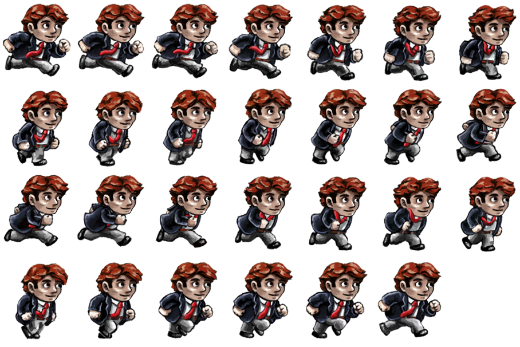
\includegraphics[width=0.2\textwidth]{example_sprite_sheet.png}
    \caption{Example sprite sheet}
    \label{fig:example_sprite_sheet}
\end{figure}

\subsection{Sprite sheet grid structure}
Sprite sheets are organized in a grid pattern.
Because all sprites are the same size the image can be divided into grid coordinates by dividing the image width by the sprite width.
In this way all sprites are able to be selected by choosing x and y coordinates and then extracting that certain part of the image.
A clear grid structure is also shown in \autoref{fig:example_sprite_sheet}.

\subsection{Showing animations}
When trying to show the animation depicted in \autoref{fig:example_sprite_sheet} it is important that the image shown to the player alternates between the images in the sprite sheet.
The speed of alternating between the images is dependent on how fast the animation is supposed to be playing.
Often times when movement between individual frames is low, the time between frames is also low.
Because objects like a player require more animations like standing, walking and jumping, it is important that more than one animation can be linked to an object and that it is possible to switch between those animations.
In extensive game engines switching between animations is handled by an animation system, animations systems are explained further in the Animation systems section.

\subsection{Animation systems}
An animation system in a game engine is the system that manages the transitions between different animations on the same object.
An engine like Unity \cite{unity} has an entire graphical animation system built into the engine like shown in \autoref{fig:unity_animation_system_overview}.
With the graphical animation system that Unity possesses it is possible to define animations, drag and drop them into the animation controller and set transition conditions.
After the initial setup, the animation system switches the shown animation and sprite automatically.

\begin{figure}[h!]
    \centering
    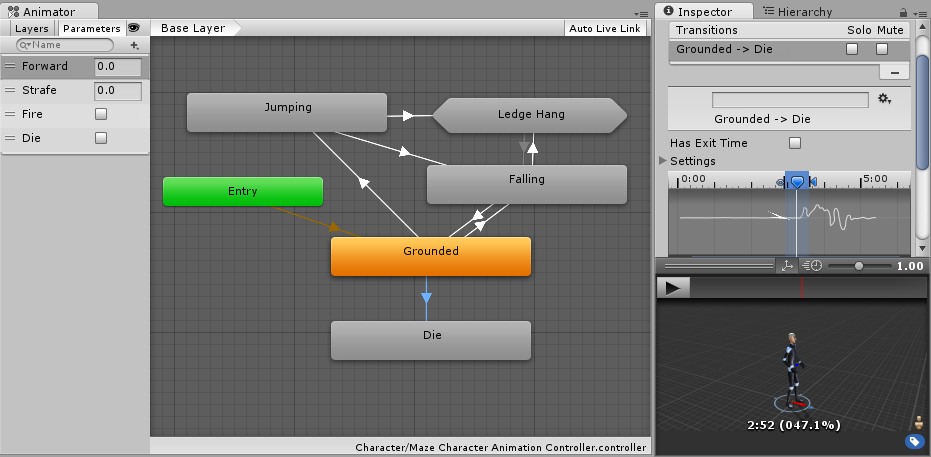
\includegraphics[width=0.9\textwidth]{unity_animation_system_overview.png}
    \caption{Unity animation system overview}
    \label{fig:unity_animation_system_overview}
\end{figure}

\subsection{Sprite atlases}
A sprite atlas class is a software component designed to handle and manage sprite sheets.
This class enables the dissection of a sprite sheet into individual sprites or animations by taking the sheet as input and logically dividing it based on specified parameters like frame width, height, and animation sequences.
By organizing and extracting these individual frames, the sprite atlas class simplifies the process of managing multiple sprites for character animations, user interface elements, or other game assets.
